\section{Theorie}
\label{sec:theorie}

Vorweg sei gesagt, dass die folgenden Überlegungen zum hier
durchgeführten Versuch aufgrund der Wechselwirkungen
zwischen Elektronen und Luftmolekülen
nur im Hochvakuum möglich sind.


\subsection{Austrittsarbeit und Energieverteilung}

Die hohe Leitfähigkeit von Metallen rührt aus ihrer kristallinen
Festkörperstruktur, in der praktisch alle Atome ionisiert sind.
So bildet sich ein periodisches Gitter, auf dem sich Elektronen 
als Leitungselektronen 'frei' bewegen können. \\

Das dabei vorherrschende Gitterpotential unterscheidet sich um
den Betrag $\Phi$ vom Außenraum und kann dabei näherungsweise
als konstant angenommen werden. \\

Möchte ein Elektron nun das Metall verlassen, muss es, wie in
\autoref{fig:abb1} dargestellt, den Potentialtopf verlassen,
sprich die Austrittsarbeit $\text{e}_0 \xi$ leisten. \\

\begin{figure}[H]
    \centering
    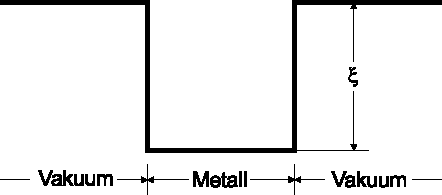
\includegraphics{figures/Abb1.pdf}
    \caption{Potentialtopfmodell eines Metalls\cite{ap09}.}
    \label{fig:abb1}
\end{figure}

Die Elektronen unterliegen dabei als Teilchen mit halbzahligem
Spin dem Pauli-Prinzip, das besagt, dass jeder mögliche
Zustand der Energie $E$ von höchstens zwei Elektronen mit
entgegengesetztem Spin eingenommen werden kann.
So besitzen Elektronen auch im absoluten Nullpunkt noch eine Restenergie,
die Fermische Grenzenergie $\zeta$. \\
Diese Grenzenergie ist bei Raumtemperatur $>> \text{k}_\text{B} T$. \\

Die Fermi-Diracsche Verteilungsfunktion beschreibt dabei die Wahrscheinlichkeit,
einen möglichen Zustand der Energie $E$ als besetzt vorzufinden. \\
Sie besitzt die Form
\begin{equation*}
    f(E) = \dfrac{1}{\text{exp}(\frac{E - \zeta}{\text{k}_\text{B} T} + 1)} \,,
\end{equation*}
ihr Verlauf ist in \autoref{fig:abb2} dargestellt.

\begin{figure}[H]
    \centering
    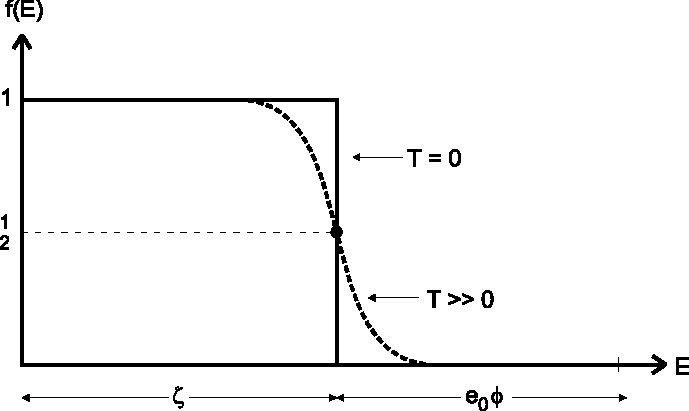
\includegraphics{figures/Abb2.pdf}
    \caption{Verlauf der Fermi-Diracschen Verteilungsfunktion am absoluten Nullpunkt \cite{ap09}.}
    \label{fig:abb2}
\end{figure}

Die dabei zum Verlassen des Metalls nötige Energie $\zeta + \text{e}_0 \Phi$
ist selbst beim Schmelzpunkt von Wolfram groß gegen $\text{k}_\text{B} \,T$,
sodass sich die Näherung
\begin{equation}
    f(E) \approx \text{exp}\left(\dfrac{\zeta - E}{\text{k}_\text{B} \, T} \right)
    \label{eq:approxfermidirac}
\end{equation}
verwenden lässt.


\subsection{Sättigungsstromdichte bei thermischer Elektronenemission}

Nun soll ein Koordinatensystem eingeführt werden, dessen z-Achse
senkrecht auf der Metalloberfläche steht. \\

Im Impulsraum ist die Zahl der Elektronen, die pro Zeit- und Flächeneinheit aus dem Volumenelement
auf die Oberfläche treffen, ist dann gegeben durch

\begin{equation}
    \dif \alpha = v_z \, n(E) \, \dif p_x \, \dif p_y \, \dif p_z \,,
    \label{eq:elekprozeitfläche}
\end{equation}

wobei $v_z$ die Elektronengeschwindigkeit in z-Richtung,
also orthogonal zur Metalloberfläche ist.
Die Zahl der Elektronen pro Volumeneinheit wird durch $n(E)$ beschrieben. \\

Unter Verwendung von
\begin{equation*}
    E = \dfrac{1}{2 \text{m}_0} \sum_{i=1}^3 p^2_i = \dfrac{\text{m}_0}{2} \sum_{i=1}^3 v^2_i
\end{equation*}
lässt sich \eqref{eq:elekprozeitfläche} schreiben als

\begin{equation}
    \dif \alpha = \dfrac{\partial E}{\partial p_z} \, n(E) \, \dif p_x \, \dif p_y 
    \, \dif p_{z} = n(E) \, \dif E \, \dif p_x \, \dif p_y \,.
    \label{eq:dalphaE}
\end{equation} \\

Dabei ist mit $f(E)$ aus \eqref{eq:approxfermidirac}
\begin{equation*}
    n(E) = \dfrac{2}{\text{h}^3} f(E) \,,
\end{equation*}
sodass sich
\begin{equation*}
    \dif \alpha = \dfrac{2}{\text{h}^3} \text{exp} \left(\dfrac{\zeta - E}{\text{k}_\text{B} \, T} \right)
                    \dif p_x \, \dif p_y \, \dif E
\end{equation*}
ergibt. \\

Die Stromdichte $j_\text{S}$ ist dann gegeben durch die Richardson-Gleichung mit
\begin{equation}
    j_\text{S} (T) = 4 \pi \dfrac{\text{e}_0 \, \text{m}_0 \, \text{k}^2_\text{B}}{\text{h}^3}
                     T^2 \text{exp} \left(- \dfrac{\text{e}_0 \Phi}{\text{k}_\text{B} \, T}\right)
    \label{eq:stromdichte}
\end{equation}
gegeben.


\subsection{Langmuir-Schottkysche Raumladungsgleichung}

Wird der Anodenstrom einer Hochvakuumdiode gemessen, lässt sich 
bei gegebener Kathodenspannung eine Abhängigkeit von der Anodenspannung feststellen.
Die Elektronen führen eine beschleunigte Bewegung in Richtung der Anode durch,
die Raumladungsdichte $\rho$ ist also ortsabhängig, da die 
Kontinuitätsgleichung
\begin{equation}
    j = - \rho \, v
    \label{eq:kontiglei}
\end{equation}
ständig erfüllt sein muss. \\

Unter Betrachtung in einer Dimension gilt die Poisson-Gleichung
\begin{equation}
    \dfrac{\dif^2 V}{\dif x^2} = - \dfrac{\rho (x)}{\epsilon_0} \,.
\end{equation}
Unter Verwendung von \eqref{eq:kontiglei} und dem Energiesatz
\begin{equation*}
    \text{e}_0 V = \dfrac{\text{m}_0}{2} \, v^2
\end{equation*}
ergibt sich nach einigen Rechenschritten
\begin{equation*}
    V(x) = \left(\dfrac{3}{4} \sqrt{\dfrac{4j}{\epsilon_0 \sqrt{\frac{2\text{e}_0}{\text{m}_0}}}} \, x \right)^{\frac{4}{3}}
    \label{eq:potential}
\end{equation*}
für das Potential $V(x)$. \\

Es wächst also nicht linear mit $x$, sondern folgt einem $x^{\frac{4}{3}}$-Gesetz. \\

Nach der Stromdichte umgestellt ergibt sich für $j$ an der Anode
\begin{equation}
    j = \dfrac{4}{9} \epsilon \sqrt{2\frac{\text{e}_0}{\text{m}_0}} \dfrac{v^{\frac{3}{2}}}{a^2} \,.
    \label{eq:anodestromdichte}
\end{equation}

Diese Gleichung wird auch als Langmuir-Schottkysche Raumladungsgleichung bezeichnet,
wobei das Potential $V(x)$, die Feldstärke $E(x)$ und die Rauladungsdichte $\rho(x)$
den in \autoref{fig:abb2} dargestellten Verläufen folgen.

\begin{figure}[H]
    \centering
    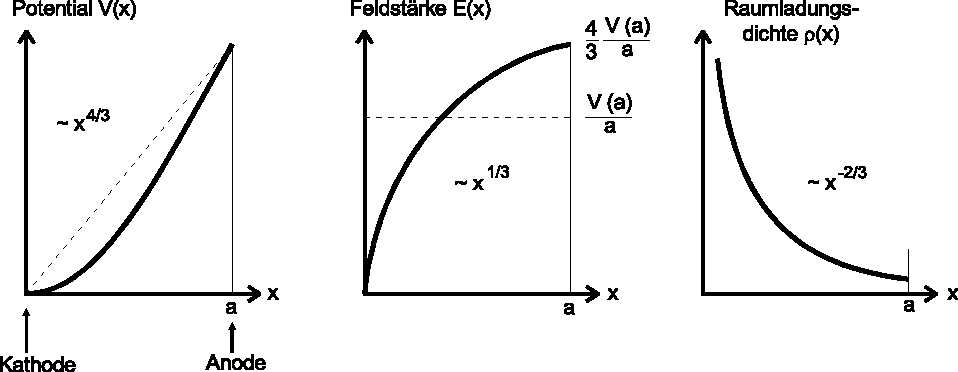
\includegraphics{figures/Abb4.pdf}
    \caption{Ortsabhängigkeiten von $V$, $E$ und $\rho$ im Raumladungsgebiet
             einer Hochvakuumdiodenkennlinie \cite{ap09}.}
    \label{fig:abb4}
\end{figure}


\subsection{Anlaufstrom einer Hochvakuumdiode}

Entgegen \eqref{eq:anodestromdichte} liegt aufgrund der Eigengeschwindigkeit der Elektronen bei Verlassen
der Kathode auch bei $V = 0$ ein geringer Anodenstrom vor.
Dabei besitzen sie den Energieüberschuss
\begin{equation*}
    \Delta E = E - (\zeta + \text{e}_0 \phi) \,,
\end{equation*}
der sich als kinetische Energie wiederfinden lässt. \\

Selbst bei einem niedrigen Gegenfeld lassen sich emittierte Elektronen beobachten,
weshalb dieser Strom auch als Anlaufstrom bezeichnet wird. \\

Das Potentialverhältnis zwischen Kathode und Anode mit der
Austrittsarbeit $\phi_\text{A} > \phi_\text{K}$ an der Anode
ist in \autoref{fig:abb5} dargestellt.

\begin{figure}[H]
    \centering
    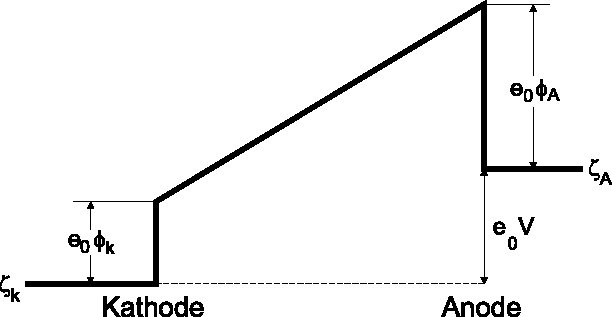
\includegraphics{figures/Abb5.pdf}
    \caption{Potentialverhältnisse in einer Hochvakuumdiode im Anlaufstromgebiet \cite{ap09}.}
    \label{fig:abb5}
\end{figure}

Die Stromdichte lässt sich also über eine Konstante $j_0$ schreiben als

\begin{equation*}
    j(V) = j_0 \, \text{exp}\left(-\dfrac{\text{e}_0 \phi_\text{A} + \text{e}_0 V}{\text{k}_\text{B} \, T} \right)
         = c \,\text{exp}\left(-\dfrac{\text{e}_0 V}{\text{k}_\text{B} T} \right)
\end{equation*}


\subsection{Kennlinie einer Hochvaluumdiode}

Der Zusammenhang zwischen Stromdichte $j$ bzw. Anodenstrom $I_\text{A}$
und dem von außen angelegten Potential wird als Kennlinie bezeichnet und lässt sich unter
den in vorangegangenen Kapiteln getroffenen Annahmen in drei, wie in \autoref{fig:abb6}
dargestellte Bereiche unterteilen.

\begin{figure}[H]
    \centering
    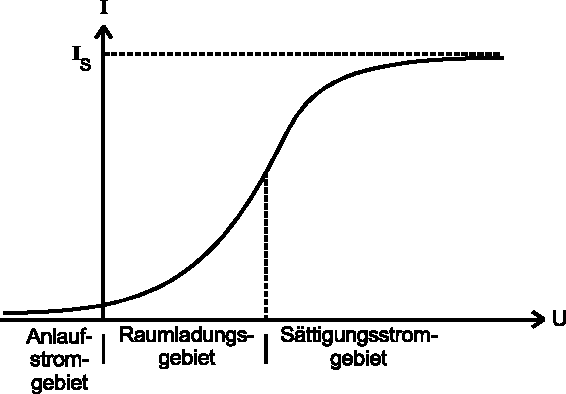
\includegraphics{figures/Abb6.pdf}
    \caption{Kennlinie einer Hochvakuumdiode \cite{ap09}.}
    \label{fig:abb6}
\end{figure}

So lässt sich im Anlaufstromgebiet $(V < 0)$ eine exponentielle und
im Raumladungsgebiet eine $\sqrt{V^3}$-Abhängigkeit beobachten.
Sättigungsstromgebiet strebt der Strom $I_\text{S}$ gegen einen
Sättigungswert.




